\phantomsection
\subsection{(10\%) Cài đặt và cấu hình dịch vụ DHCP trên server để cấu hình mạng tự động
  cho các máy desktop trong nhánh mạng}

\begin{itemize}
  \item[--] Địa chỉ IP của desktop: trong dãy 10.0.2.50/24 đến 10.0.2.100/24
  \item[--] Địa chỉ gateway:  10.0.2.1
  \item[--] DNS server: 10.0.2.2 và 8.8.8.8
\end{itemize}

\phantomsection
\subsubsection{Cài đặt dịch vụ DHCP}
\begin{minipage}{.93\linewidth}
  \captionsetup{type=figure, skip=-15pt}
  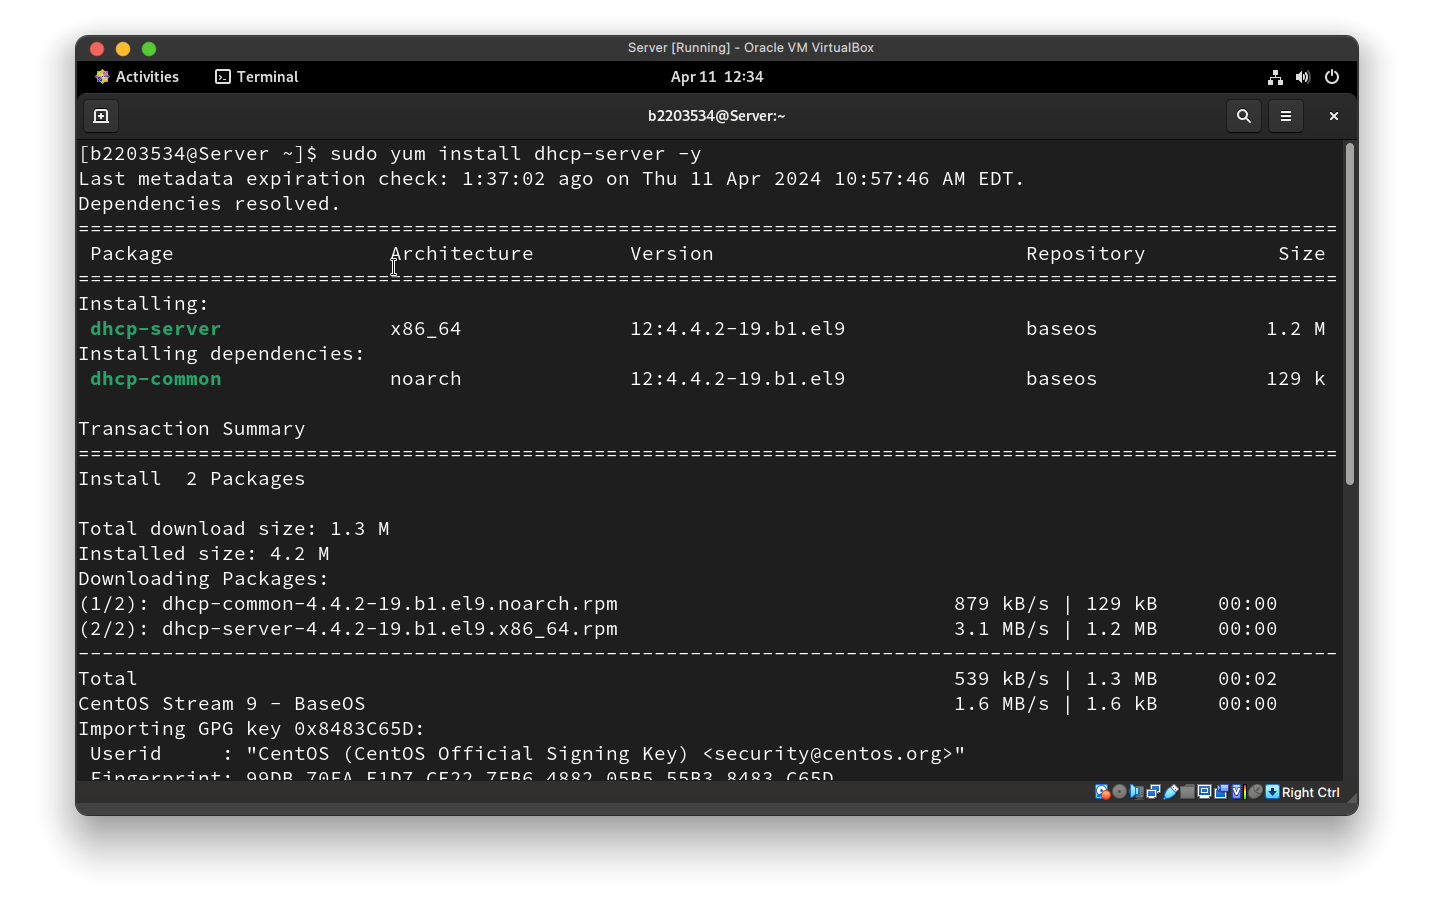
\includegraphics[width=\linewidth]{./imgs/image51.png}
  \caption{\bfseries Cài đặt dịch vụ \texttt{dchp-server}}
\end{minipage}

\vspace{0.5cm}
\begin{bashlisting}{Cài đặt dịch vụ \texttt{dchp-server}}
  sudo yum install dhcp-server -y
\end{bashlisting}

\phantomsection
\subsubsection{Cấu hình dịch vụ DHCP}

Ta chỉnh sửa nội dung file \texttt{/etc/dhcp/dhcpd.conf} để cấu hình dịch vụ DHCP
\textit{(\myref{fig:config-dhcp})}.

\begin{minipage}{.93\linewidth}
  \captionsetup{type=figure, skip=-15pt}
  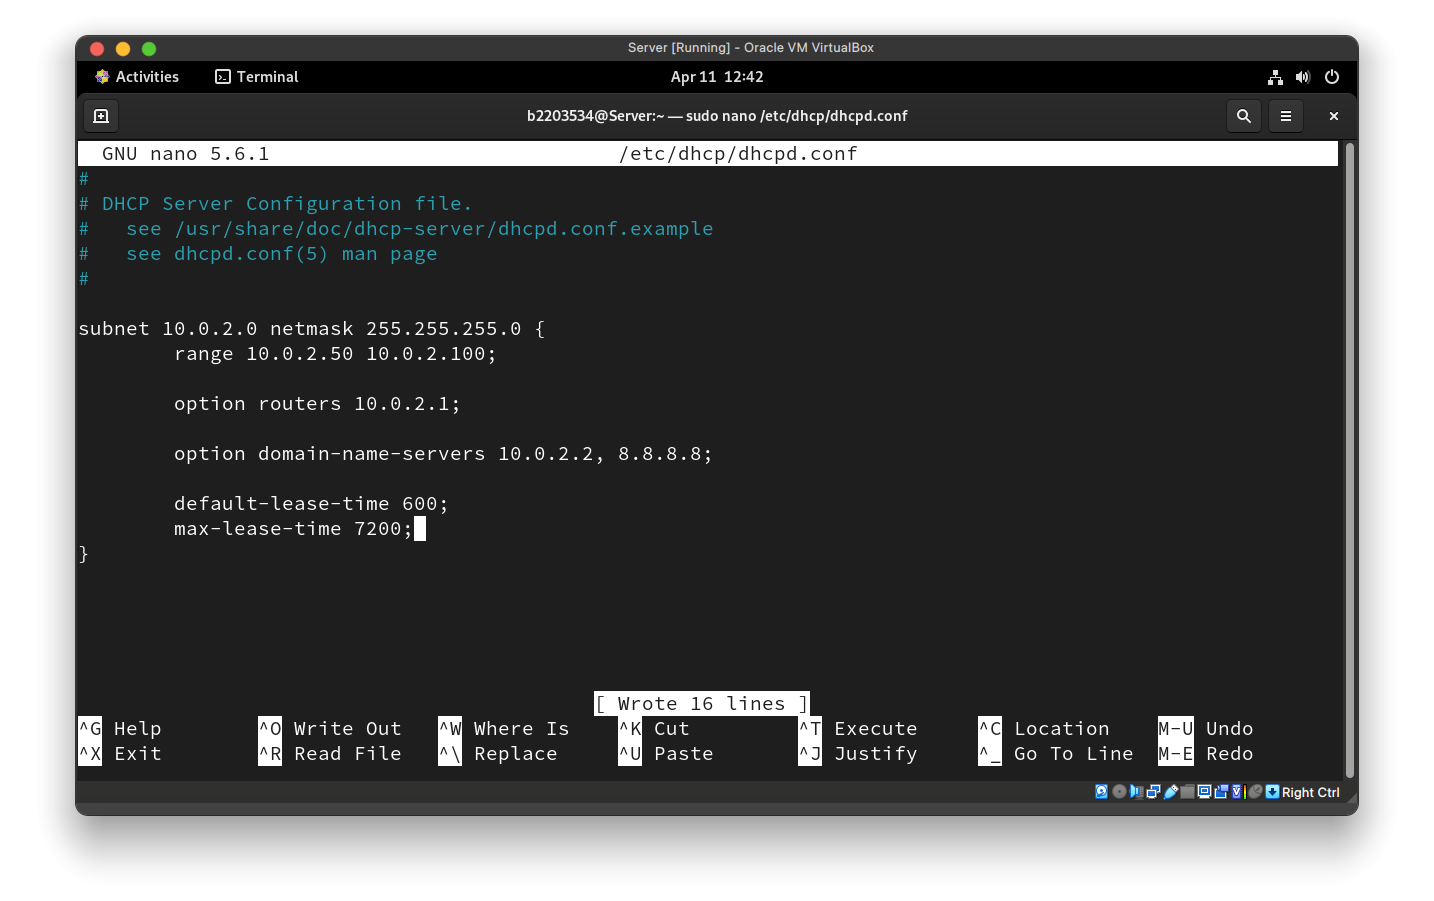
\includegraphics[width=\linewidth]{./imgs/Hinh-18.png}
  \caption{\bfseries Cấu hình dịch vụ DHCP}
  \label{fig:config-dhcp}
\end{minipage}

Nội dung file \texttt{/etc/dhcp/dhcpd.conf} như sau:

\vspace{0.5cm}
\begin{bashlisting}{Cài đặt dịch vụ \texttt{dchp-server}}
  subnet 10.0.2.0 netmask 255.255.255.0 {
      range 10.0.2.50 10.0.2.100;

      option routers 10.0.2.1;

      option domain-name-servers 10.0.2.2, 8.8.8.8;

      default-lease-time 600;
      max-lease-time 7200;
    }
\end{bashlisting}

\begin{itemize}
  \item [\textbf{Dòng 1}] Cấu hình subnet là 255.255.255.0 với địa chỉ mạng là 10.0.2.0.
  \item [\textbf{Dòng 2}] Cấu hình range địa chỉ IP cho các máy desktop là từ 10.0.2.50 đến 10.0.2.100.
  \item [\textbf{Dòng 4}] Cấu hình địa chỉ gateway là 10.0.2.1.
  \item [\textbf{Dòng 6}] Cấu hình địa chỉ DNS server là 10.0.2.2, 8.8.8.8.
  \item [\textbf{Dòng 8}] Cấu hình thời gian mặc định mà một thiết bị sẽ được cấp phát địa chỉ IP là 600s.
  \item [\textbf{Dòng 9}] Cấu hình thời gian tối đa mà một thiết bị được cấp địa chỉ IP là 7200s (2h).
\end{itemize}

\phantomsection
\subsubsection{Khởi động dịch vụ DHCP}
\begin{minipage}{.93\linewidth}
  \captionsetup{type=figure, skip=-15pt}
  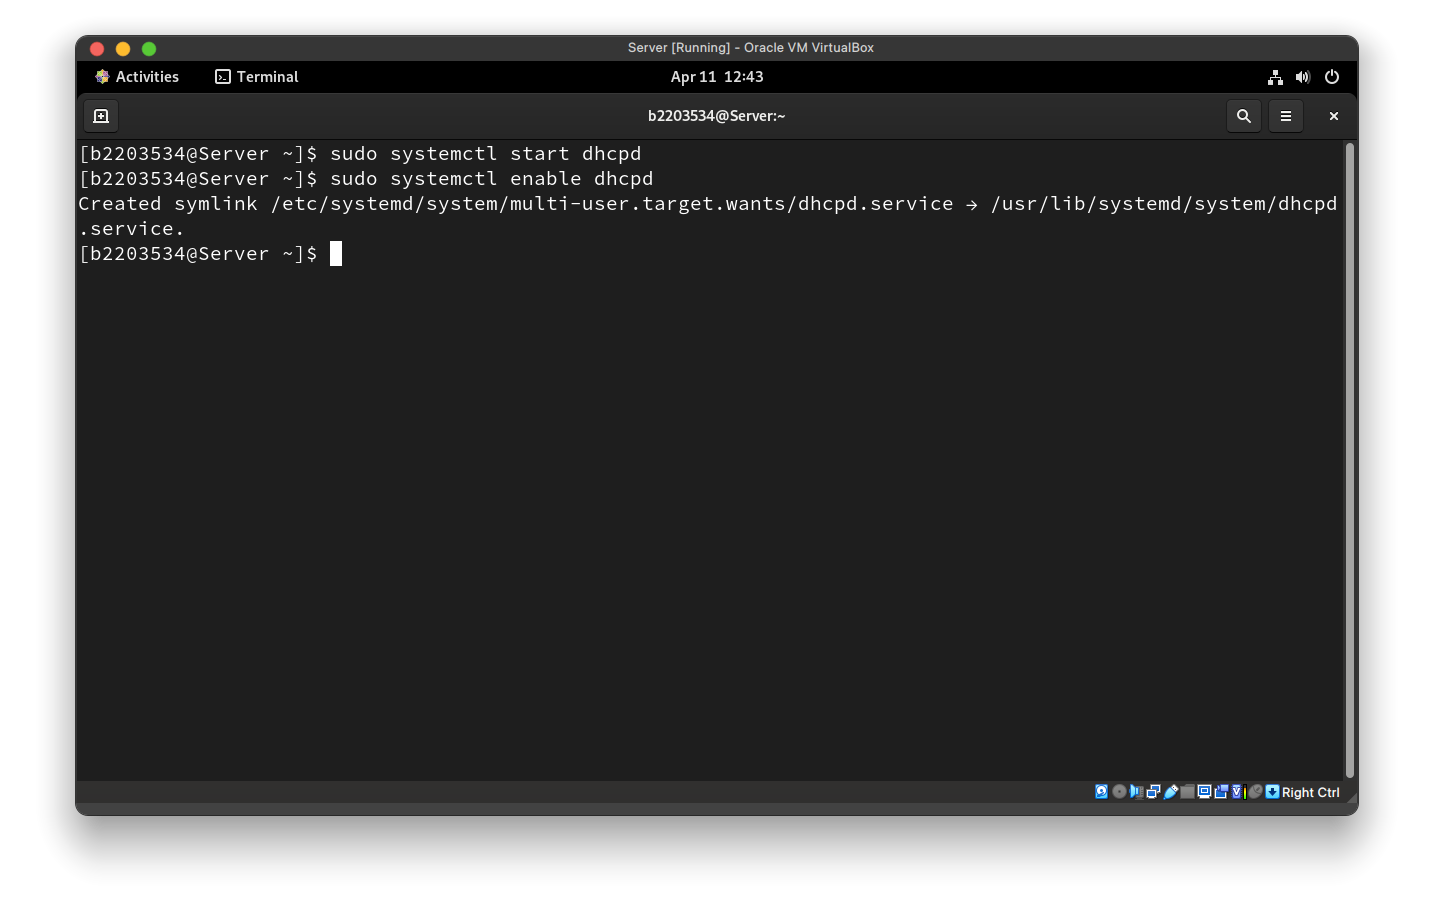
\includegraphics[width=\linewidth]{./imgs/Hinh-19.png}
  \caption{\bfseries Khởi động dịch vụ DHCP}
\end{minipage}

\vspace{0.5cm}
\begin{bashlisting}{Khởi động dịch vụ DHCP}
  sudo systemctl start dhcpd
  sudo systemctl enable dhcpd
\end{bashlisting}

\phantomsection
\subsubsection{Kiểm tra dịch vụ DHCP}

Sau khi cấu hình xong DHCP, ta sẽ dùng máy desktop \textit{(\myref{fig:access-website})} để kiểm tra bằng cách kết nối vào mạng \texttt{QTHT} và kiểm tra địa chỉ \texttt{IP}
của máy desktop \textit{(\myref{fig:check-ip})}.

\begin{minipage}{.93\linewidth}
  \captionsetup{type=figure, skip=-15pt}
  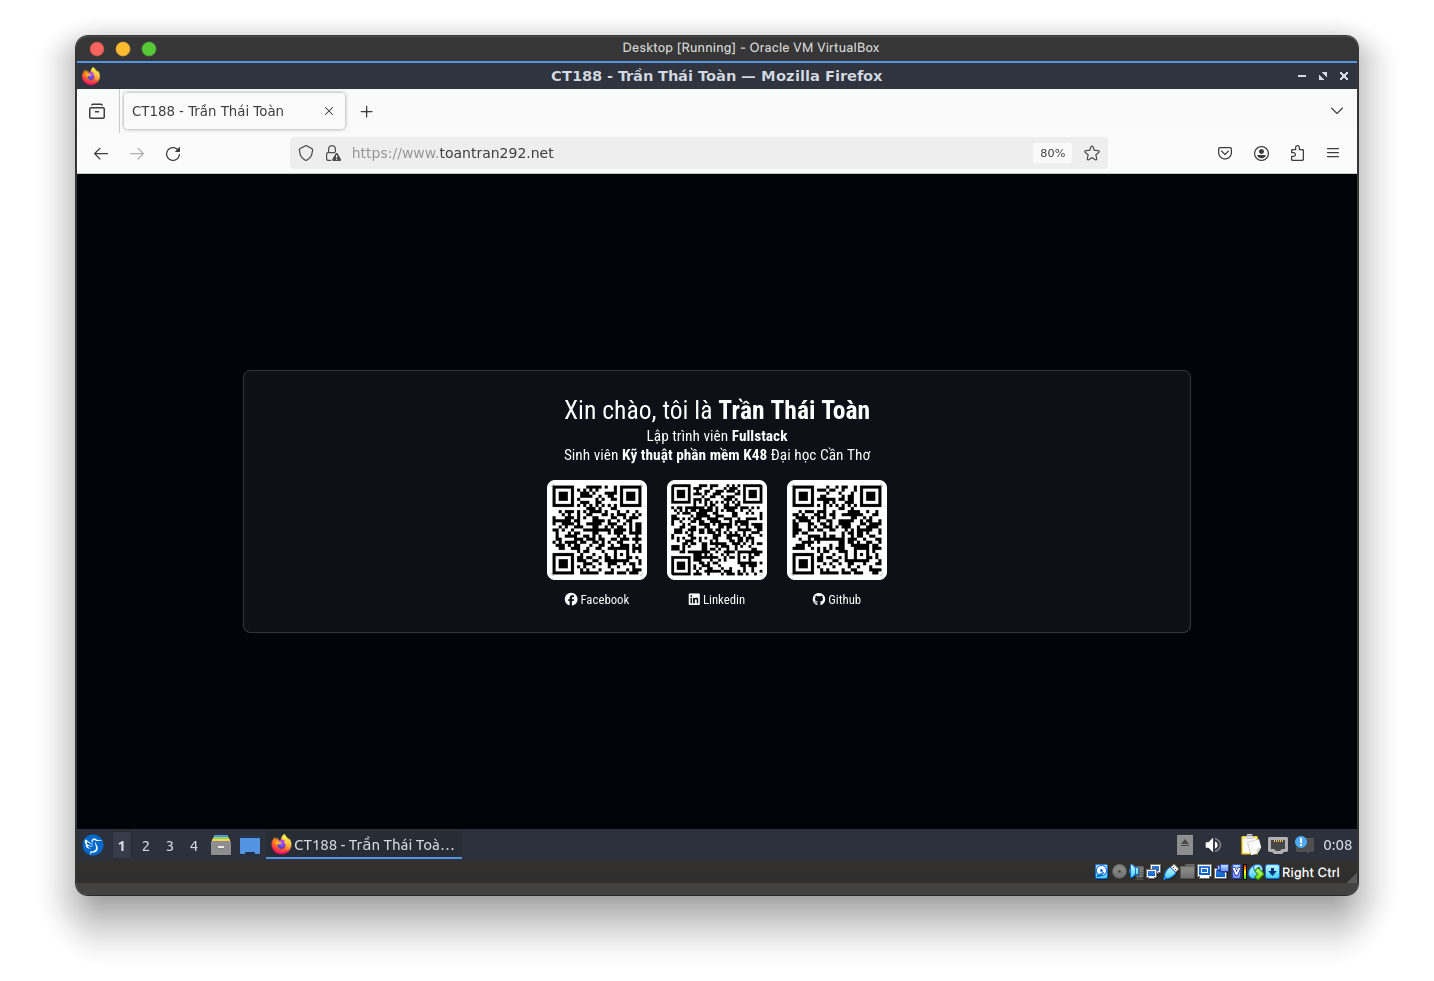
\includegraphics[width=\linewidth]{./imgs/Hinh-20.png}
  \caption{\bfseries Truy cập vào internet bằng máy desktop}
  \label{fig:access-website}
\end{minipage}

\begin{minipage}{.93\linewidth}
  \captionsetup{type=figure, skip=-15pt}
  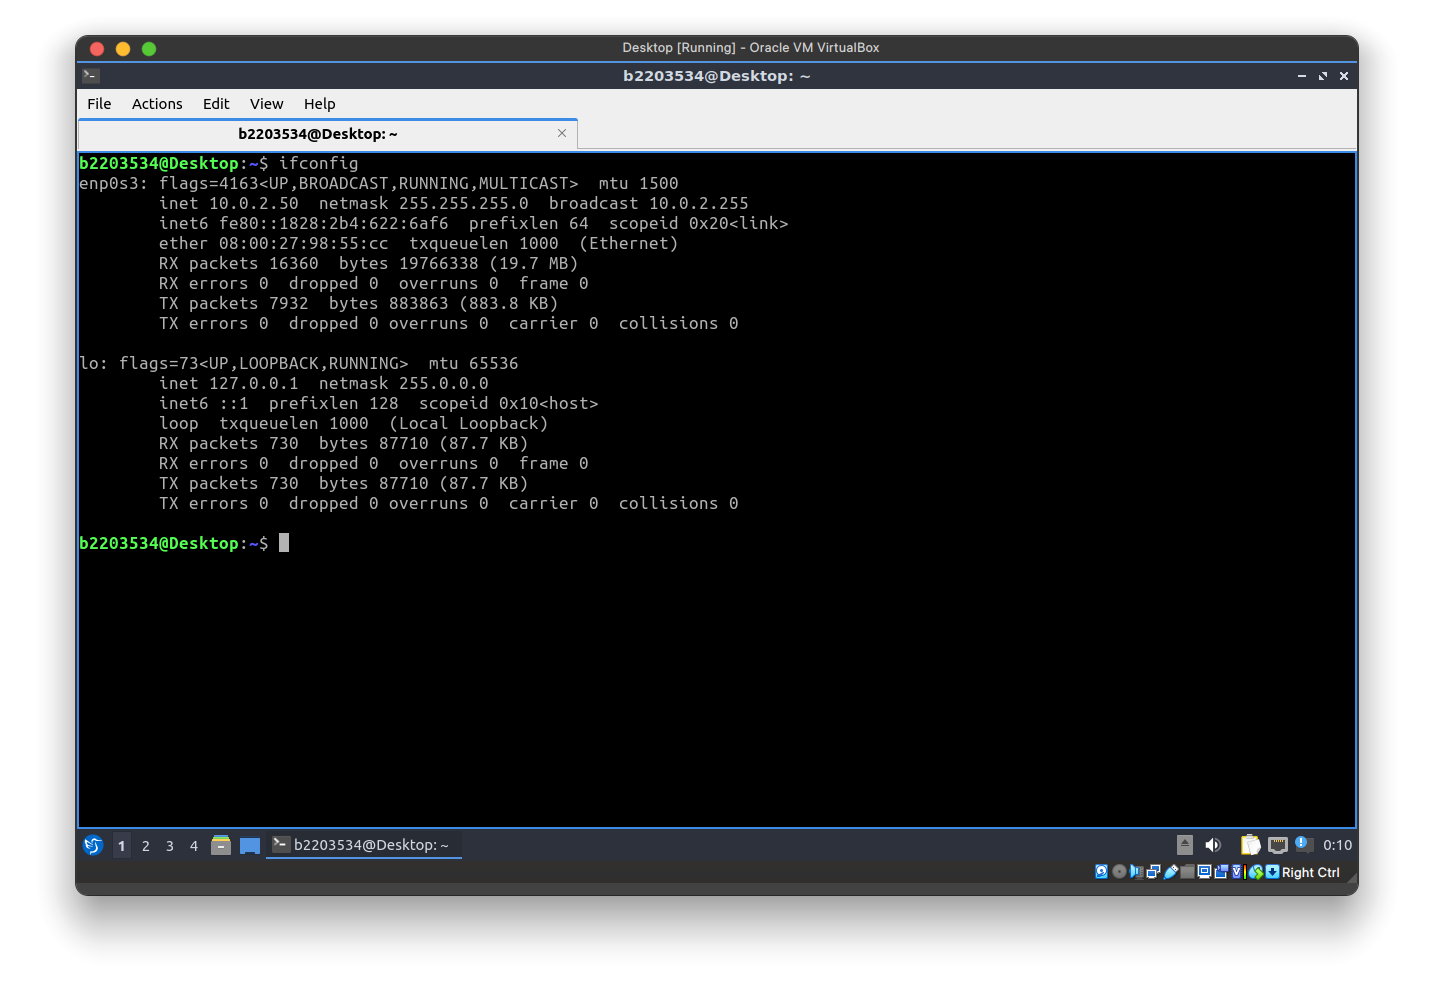
\includegraphics[width=\linewidth]{./imgs/Hinh-21.png}
  \caption{\bfseries Kiểm tra địa chỉ IP của máy desktop (10.0.2.50)}
  \label{fig:check-ip}
\end{minipage}
